\documentclass[a4paper,fleqn]{cas-sc}

\usepackage[numbers]{natbib}
\usepackage{amsmath,amssymb,mathtools}
\usepackage{booktabs}
\usepackage{enumitem}
\usepackage{graphicx}
  \graphicspath{{./}{graphics/}}
\usepackage{url}

%%%%%%%%%%%%%%%%%%%%%%%% DEFINITIONS %%%%%%%%%%%%%%%%%%%%%%%%%%

\newcommand{\asrt}{\mathbin{\text{!}}}
\newcommand{\typeof}[1]{\tau(#1)}
\newcommand{\abs}[1]{\left|#1\right|}

\newcounter{majorcount}
\newcounter{minorcount}[majorcount]

\newcommand{\deffy}[3]{
	\vspace{2ex}
	\refstepcounter{majorcount}
	\noindent\textsc{#1}
	\\\begin{small}
	\noindent #2%
	\label{Def:#3}
	\end{small}
	\vspace{2ex}
}

\newlist{criteria}{enumerate}{1}
\setlist[criteria,1]{
  label=\footnotesize{\arabic*},
  leftmargin=*,
  align=left,
  labelsep=1em,
}

%%%%%%%%%%%%%%%%%%%%%%%%%%%%%%%%%%%%%%%%%%%%%%%%%%%%%%%%%%%%%%%%

\begin{document}
\let\WriteBookmarks\relax
\def\floatpagepagefraction{1}
\def\textpagefraction{.001}

\shorttitle{Transitional Representation}
\shortauthors{L. R\"onnb\"ack}

\title[mode=title]{Transitional Representation: A Formalism for Conflicting and Evolving Data}
\tnotemark[1]
\tnotetext[1]{Initial rework --- 4 March 2026.}

\author[1]{Lars R\"onnb\"ack}
\cormark[1]
\ead{lars@anchormodeling.com}
\affiliation[1]{organization={Anchor Modeling},
                country={Sweden}}
\cortext[cor1]{Corresponding author}

\begin{abstract}
Modern information systems increasingly need to represent information that is concurrent (multiple sources and perspectives), bitemporal (what was believed when, about what happened when), and uncertain (graded confidence and explicit disagreement). Existing representation formalisms typically handle at most one or two of these dimensions without either losing provenance or forcing early conflict resolution. This paper proposes \emph{transitional representation}, a formalism whose atomic units are \emph{posits} (\(n\)-ary, time-stamped statements) and \emph{assertions} (time-stamped, signed certainties about posits). We further give a deterministic bitemporal selection procedure (\emph{information in effect}) that defers conflict resolution to query time while retaining full history.
\end{abstract}

\begin{keywords}
transitional \sep posit \sep assertion \sep bitemporality \sep concurrency \sep uncertainty
\end{keywords}

\maketitle

\section{Introduction}
\noindent\textbf{The problem} is not that databases cannot store facts, but that they routinely discard the circumstances of those facts: who stated them, how confident they were, when the statement was recorded, and how both the world and opinions about it change over time. Modeling these requirements explicitly in conventional designs is complex and therefore often omitted, producing lossy implementations and lost provenance \cite{GolfarelliRizzi}. Yet in practice, statements have origins and degrees of confidence \cite{Liu}, and many domains require full auditability and non-destructive history (e.g., regulated finance, clinical records, intelligence and judicial applications) \cite{FisherEtAl}.

\noindent
Even when temporal support exists at the database level, it is typically layered onto the relational model and remains insufficient for representing multi-source disagreement and evolving beliefs \cite{SQL2011,Johnston}. A central motivation in this paper is to move conflict handling from \emph{write time} (where integration rules prematurely discard alternatives) to \emph{query time} (where decisions can be made using the full body of competing evidence) \cite{MassaroEtAl,LinEtAl}.

\noindent
We use the following running example throughout:
\begin{quote}
\small
The accused, Archie, was seen fleeing the scene of the crime by two witnesses, Donna and Charlie. Donna is certain that the accused was clean shaved, while Charlie thinks he had a red beard. When the victim, Bella, later regained consciousness, she corroborated Charlie's story, at which time Donna retracted her statement. In fact, Archie had been wearing a fake red beard during the attack, but it fell off when he fled, eventually leading to his conviction through a DNA match.
\end{quote}

\noindent
\textsc{Contributions.} This rework focuses narrowly on: (i) the posit/assertion duality as the atomic representation construct, (ii) a signed certainty scale \(c\in[-1,1]\), and (iii) the bitemporal algorithm for selecting the \emph{information in effect}. Topics like schema bootstrapping, identification, and constraint enforcement are deferred to future work.

\section{The Transitional Model (Core Constructs)}
\subsection{Posits}
\deffy{def. of an appearance and a role}{%
An \emph{appearance} is a pair \((i, r)\) where the first element is a unique identifier and the second a string called \emph{role}.}{appearance}

\noindent
\textbf{Note on identifiers.} Identifiers are opaque tokens: the formalism receives them as the \emph{outcome} of an identification process that operates entirely outside the representation layer. Identification is a search process by which circumstances are matched against available data, ending in one of two outcomes: an identity is established or it is not. What those circumstances are may vary widely --- from a reproducible customer-number lookup to an open-ended detective investigation. When the process is so reproducible that the same circumstances always produce the same result, those circumstances constitute a \emph{key}. Keys are useful automation aids for the identification process, but they must never affect the representation model itself: a model that encodes a particular identification process would reflect a single point of view, be bound to the time frame in which that process is valid, and risk obsolescence when the process changes.

\noindent
Identifiers are, however, the one element that positors must share to be in genuine conflict---two positors can only disagree if their assertions reference the same appearance set, which requires agreed-upon referents. Everything else concerning an entity remains expressible \emph{within} the formalism as ordinary posits with reserved roles: classification (``J42 is a person since 1980-02-13''), class transitions (``J42 is a female child'' until ``J42 is a female adult''), and even conflicting co-reference hypotheses (``J42 and K99 refer to the same individual'', asserted with some certainty by one positor and disputed by another) are all posits subject to the usual assertion mechanics.

\deffy{def. of an appearance set}{%
An \emph{appearance set}, \(\{(i_1, r_1), \ldots (i_n, r_n)\}\), is a set of appearances where any role \(r_i\) may only appear once.}{appearanceset}

\deffy{def. of a posit}{%
A \emph{posit}~\cite{Oxford} is a triple, \(\left[D, v, t_{\mathrm{app}}\right]\), where the first element is an appearance set, the second a data value, and the third a time point. The domain \(\mathbb{t}\) from which time points are taken is called \emph{appearance time}.}{posit}

\noindent
\textbf{Interpretation.} A posit states that an appearance set \(D\) has value \(v\) from (and including) appearance time \(t_{\mathrm{app}}\) onward, until another posit with the same appearance set becomes applicable. Appearance sets are permanent anchors of change: they remain in the body of information indefinitely, even after the entities they reference no longer exist, because history must remain queryable.

\noindent
Appearance sets of size one act like \emph{properties}; appearance sets of size greater than one act like \emph{relationships}. For example:
\begin{align*}
[\{(A, \textit{has beard})\}, \textrm{fluffy red}, \textrm{10:00}] \\
[\{(A, \textit{has beard})\}, \textrm{shaved clean}, \textrm{10:02}]
\end{align*}

\noindent
and, for a relationship:
\begin{align*}
[\{(A, \textit{is accused}), (B, \textit{is victim}), (C, \textit{is witness})\}, \textrm{at scene of crime}, \textrm{09:58}] \\
[\{(A, \textit{is accused}), (B, \textit{is victim}), (C, \textit{is witness})\}, \textrm{dispersed}, \textrm{10:02}]
\end{align*}

\noindent
\textbf{Why posits are not enough.} It is tempting to model \emph{corrections} as additional posits. For instance, if a birth date was recorded incorrectly, one might add a later posit with a different value. But posits form an unordered set: there is no built-in mechanism for one posit to override another. When two posits share the same appearance set and appearance time but carry different values, the collection is ambiguous---there is no way, from inside the set of posits alone, to determine which corresponds to the actual state of affairs.\footnote{Think of posits as a shuffled deck of cards handed to you; you must identify the true ones using only the information printed on the cards themselves---no card can designate itself as the authoritative one.} Interpreted as a natural transition, conflicting same-time posits would imply the impossible: that Archie was actually born in August \emph{and} in September. Corrections must therefore be handled at a different level, by expressing evolving \emph{opinions} about posits rather than by adding rival posits.

\subsection{Assertions as Posits}
\noindent
Posits are treated as syntactical items towards which different actors may hold different and evolving opinions. To bring posits meaning while keeping a uniform representation, assertions are represented as posits themselves---meta-posits that bind a posited statement to a \emph{positor}, a signed certainty, and an assertion time.

\deffy{def. of an assertion}{%
An \emph{assertion} is a posit on the form
$$\left[\{(p_{id}, \textit{posit}), (s_{id}, \textit{ascertains})\}, c, T_{\mathrm{ast}}\right]$$
where \(p_{id}\) identifies the posit being asserted, \(s_{id}\) identifies the \emph{positor}, \(T_{\mathrm{ast}}\in\mathbb{T}\) is \emph{assertion time}, and \(c\in[-1,1]\) is \emph{signed certainty}.}{assertion}

\noindent
We write this compactly as \(\asrt(s_{id}, p_{id}, c, T_{\mathrm{ast}})\).

\noindent
Representing assertions as posits is deliberate: because an assertion is itself a posit, it can in turn be asserted by another positor, enabling recursive layers of meta-commentary—uncertainty about uncertainty, provenance of provenance—within the same uniform construct and without any change of representation.

\noindent
Intuitively, \(c=1\) means the positor is certain the posit holds, \(c=0\) means complete uncertainty, and \(c=-1\) means the positor is certain the posit does \emph{not} hold.

\noindent
Signed certainty can be read in two complementary ways: either as a number attached to a posit, or as a way to refer to the \emph{complement} of a posit (e.g., ``not shaved clean''). In practice, both are useful: complements are convenient for human communication, while signed certainty is convenient for compact storage and algebraic manipulation.

\noindent
In the running example, let:
\begin{alignat*}{3}
p_{1} = [\{(A, \textit{has beard})\},\;&& \textrm{fluffy red},\;&& \textrm{10:00}] \\
p_{2} = [\{(A, \textit{has beard})\},\;&& \textrm{shaved clean},\;&& \textrm{10:02}] \\
\asrt(C, p_{1},\;&& 0.75,\;&& \textrm{Friday}) \\
\asrt(D, p_{2},\;&& 1.0,\;&& \textrm{Friday})
\end{alignat*}

\section{Epistemic Properties of the Model}
\noindent
\textbf{Imprecision versus uncertainty.} Two distinct concepts govern how a posit relates to the world. \emph{Imprecision} is a property of values: a value such as \textit{fluffy red} maps crisply to a range of real-world colors, and whether a particular color falls within that range is an objective evaluation performed by the asserter at assertion time. \emph{Uncertainty}, by contrast, is subjective and contextual: it is the degree of belief a positor holds towards a posit, given their own information and viewpoint. A positor may be completely certain about an imprecise value (asserting \(c=1\) for ``approximately noon'' without knowing the exact minute) and completely uncertain about a precise one (asserting \(c=0\) for an exact timestamp). This distinction explains why signed certainty is subjective and can be negative—the positor is certain of the \emph{complement}—whereas a classical probability is objective and bounded below by zero.

\subsection{A signed certainty scale}
\noindent
Humans often communicate confidence linguistically rather than numerically. Table~\ref{Table:certainties2} suggests a coarse mapping\footnote{Any mapping of natural-language hedges to numerical probabilities is inherently subjective. The values here serve as a pragmatic baseline; practitioners may calibrate them for their domain. Analogous scales appear in intelligence analysis~\cite{Kent} and in the IPCC uncertainty vocabulary~\cite{IPCC}.}. 

\begin{table}[htb]
\centering
\small
\begin{tabular}{r l}
\toprule
\(c\) & Linguistic correspondence \\ \midrule
$1.00$   & It is certain that the value is $v$ \\
$0.75$   & It is probable that the value is $v$ \\
$0.50$   & It may be that the value is $v$ \\
$0.25$   & It is possible that the value is $v$ \\
$0.00$   & It could be any value whatsoever \\
$-0.25$  & It is possible that the value is not $v$ \\
$-0.50$  & It may be that the value is not $v$ \\
$-0.75$  & It is probable that the value is not $v$ \\
$-1.00$  & It is certain that the value is not $v$ \\
\bottomrule
\end{tabular}
\caption{Suggested signed certainty values and linguistic correspondences.}
\label{Table:certainties2}
\end{table}

\begin{figure}[pos=htbp]
\centering
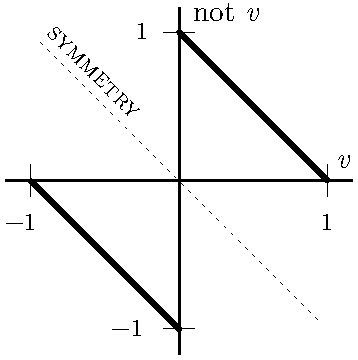
\includegraphics[width=0.25\linewidth]{v_and_not_v.pdf}
\caption{Signed certainty for a value $v$ and its negation \emph{not} $v$.}
\label{Figure:boundsym}
\end{figure}

\subsection{Well-behaving bodies of information}
\deffy{def. of a body of information}{%
A \emph{body of information} is a set of assertion posits that represent actual facts in the universe of discourse.}{body}

\noindent
A body of information is \emph{well-behaving} when its assertions satisfy a set of mutually reinforcing properties. The first ensures that negated values and negative certainties are interchangeable:

\deffy{def. of symmetric}{%
A body of information is said to be \emph{symmetric} iff the assertions \(\asrt(S, p, {-c}, T)\) and \(\asrt(S, \bar{p}, c, T)\) are equivalent for a posit \(p\) and its complement \(\bar{p}\).}{symmetry}

\noindent
Symmetry allows a positor to express ``certainly not fluffy red'' either as certainty \(-1\) for \(p\!=\)[\ldots, \textit{fluffy red}, \ldots] or as certainty \(1\) for \(\bar{p}\!=\)[\ldots, \textit{not fluffy red}, \ldots]. To avoid storing complemented values, any symmetrical body can be normalized:

\deffy{def. of canonical}{%
A body of information is said to be \emph{canonical} iff all assertions are made against posits with non-negated values.}{canonical}

\noindent
The next property bounds the certainties for a value and its complement so they cannot independently saturate the scale:

\deffy{def. of bounded}{%
A body of information is said to be \emph{bounded} iff the certainties in the assertions \(\asrt(S, p, c, T)\) and \(\asrt(S, \bar{p}, d, T)\) satisfy \(\abs{c + d} = \abs{c + d}^2\), i.e.\ \(c + d \in \{-1, 0, 1\}\).}{boundary}

\noindent
For example, if Charlie asserts \(c = 0.75\) for ``fluffy red'', boundary implies \(d = 0.25\) for ``not fluffy red''. The symmetry and bounded conditions on the certainty scale are illustrated in Figure~\ref{Figure:boundsym}. The next property prevents a positor from simultaneously holding two different certainties for the very same posit:

\deffy{def. of exclusive}{%
A body of information is said to be \emph{exclusive} iff no two assertions by the same positor for the same posit differ only in certainty.}{exclusive}

\noindent
Exclusivity rules out statements such as ``I think Archie had a red beard and I am also sure he had a red beard''. Even though the certainties \(-0.25\) and \(0.75\) for a posit are equivalent via symmetry, only one should persist. The final individual property requires that all positors share the same interpretation of appearances:

\deffy{def. of universal}{%
A body of information is said to be \emph{universal} iff positors agree on all appearances.}{universal}

\noindent
Without universality, disagreement is meaningless: positors must share a common referent to be genuinely in conflict. Together, the four properties yield:

\deffy{def. of comprehensive}{%
A body of information is said to be \emph{comprehensive} iff it is symmetric, canonical, bounded, exclusive, and universal.}{comprehensive}

\noindent
From here on all bodies of information are assumed to be comprehensive. In a concrete implementation such as Positorium~\cite{Positorium}, these properties serve as integrity constraints: the system normalises symmetric statements into canonical form and rejects assertions that would violate exclusivity or boundary rules. They can equally be applied as diagnostic criteria to audit an existing body of information. Two further properties pertain to the \emph{information in effect} rather than to individual assertions:

\deffy{def. of decisive and indecisive}{%
When multiple assertions by the same positor are in effect for posits with the same appearance set but different values, that positor is \emph{indecisive} with respect to that appearance set; when exactly one such assertion is in effect, the positor is \emph{decisive}. A body of information is \emph{decisive} if no indecisive positor exists in any information in effect, and \emph{indecisive} otherwise.}{decisiveness}

\noindent
A traditional relational database is always decisive: it permits at most one value per attribute at any given time. In transitional representation, indecisiveness is a valid and often informative state. A decisive body is always non-contradictory; in the general case, the following inequality must hold:

\deffy{def. of non-contradictory}{%
A body of information is said to be \emph{non-contradictory} iff for every information in effect the certainties across all concurrent assertions by the same positor for the same appearance set satisfy
$$|\{i \mid c_i < 0\}| + \sum_{i=1}^{n}c_i\leq 1,$$
where $|\{i \mid c_i < 0\}|$ counts the number of negative certainties in the set.}{noncontradiction}

\noindent
\textsc{Derivation.} The formula follows from the requirement that the total \emph{positive commitment} across mutually exclusive alternatives must not exceed~1. For a positive certainty $c_i > 0$, the positor claims $c_i$ units of certainty that value $v_i$ holds. For a negative certainty $c_j < 0$, the positor claims $|c_j|$ certainty that $v_j$ does \emph{not} hold; by the bounded property this implicitly allocates $1 - |c_j| = 1 + c_j$ units of certainty toward the set of all other alternatives. Summing both types of commitment gives:
$$\sum_{c_j < 0}(1 + c_j) + \sum_{c_i > 0}c_i = |\{i \mid c_i < 0\}| + \sum_{i=1}^{n}c_i.$$
Requiring this total not to exceed~1 prevents the positor from collectively over-committing across mutually exclusive alternatives. When all certainties are non-negative the formula reduces to the classical budget constraint $\sum c_i \leq 1$; asserting $c_j=-1$ (``certainly not $v_j$'') contributes zero to the budget (since $1 + (-1) = 0$), so a positor may freely disbelieve any number of values without tightening the constraint on their positive claims.

\noindent
\textsc{Example.} Suppose Donna has two assertions simultaneously in effect at \((\textrm{Sunday}, \textrm{10:03})\):
\[a_5 = \asrt(D,\,p_4,\;0.25,\;\textrm{Sunday})\quad\text{and}\quad a_6 = \asrt(D,\,p_2,\;{-0.75},\;\textrm{Sunday})\]
(``possibly fluffy red'' and ``probably not shaved clean''). One certainty is negative ($-0.75$), and the sum is $0.25 + (-0.75) = -0.5$, so the left-hand side equals $1 + (-0.5) = 0.5 \leq 1$. Donna is well within bounds and is not contradicting herself. Note that a positor may simultaneously assert \(c=-1\) (``certainly not'') for an unlimited number of posits without ever violating the inequality.

\noindent
\textsc{Mutual exclusivity.} The non-contradiction formula applies per appearance set and assumes that the posits being compared represent \emph{mutually exclusive} alternatives for a single value slot. ``Archie's beard is fluffy red'' and ``Archie's beard is shaved clean'' are alternatives for the same appearance set \(\{(A, \textit{has beard})\}\), so they compete. If a domain requires multi-valued attributes, each value dimension must be separated into distinct roles so that each appearance set carries exactly one value at a time --- the functional dependency from appearance set to value is a design requirement, not an incidental restriction.

\section{Bitemporal Dynamics (Information in Effect)}
\subsection{Retractions and corrections}
\deffy{def. of complete uncertainty}{%
An assertion posit is called \emph{completely uncertain} when the signed certainty is $0.0$.}{uncertain}

\deffy{def. of a retraction}{%
Let \(\mathbb{A}\) be a body of information. A \emph{retraction} is an assertion posit
\(\left[\{(p_{id}, \textit{posit}), (s_{id}, \textit{ascertains})\}, 0.0, T'\right] \in \mathbb{A}\)
for which there exists an earlier assertion
\(\left[\{(p_{id}, \textit{posit}), (s_{id}, \textit{ascertains})\}, c, T\right] \in \mathbb{A}\)
with \(c\neq 0\) and \(T < T'\).}{retraction}

\deffy{def. of a correction}{%
Let \(\mathbb{A}\) be a body of information. The three assertion posits
\(a_1 = \left[\{(p_{id}, \textit{posit}), (s_{id}, \textit{ascertains})\}, c, T\right]\),
\(a_2 = \left[\{(p_{id}, \textit{posit}), (s_{id}, \textit{ascertains})\}, 0.0, T'\right]\), and
\(a_3 = \left[\{(p'_{id}, \textit{posit}), (s_{id}, \textit{ascertains})\}, c', T'\right]\)
form a \emph{correction} when \(p_{id} \neq p'_{id}\), \(c\neq 0\), \(c'\neq 0\), and \(T < T'\).}{correction}

\subsection{The information in effect}
\deffy{def. of the information in effect}{%
Let \(\mathbb{A}\) be a body of information. The \emph{information in effect} is a subset
\(\mathbb{A}(T_@, t_@) \subset \mathbb{A}\)
given a bitemporal point \((T_@, t_@) \in \mathbb{T} \times \mathbb{t}\).
Assuming \(s_{id}\), \(c\), \(T\), \(D\), \(v\), and \(t_{\mathrm{app}}\) are free variables, all assertion posits
\(\left[\{(p_{id}, \textit{posit}), (s_{id}, \textit{ascertains})\}, c, T\right] \in \mathbb{A}(T_@, t_@)\)
with posit \(p = [D, v, t_{\mathrm{app}}]\) are found using the following selection criteria:
\begin{criteria}
\item Let \(\mathbb{A}_1 \subset \mathbb{A}\) be the assertions satisfying \(T \leq T_@\) and \(t_{\mathrm{app}} \leq t_@\).
\item Let \(\mathbb{A}_2 \subset \mathbb{A}_1\) be the assertions with \(c \neq 0\) and the latest appearance time \(t_{\mathrm{app}}\) for each combination of \(s_{id}\) and \(D\), excluding those for which a retraction exists at some \(T_0\) with \(T \leq T_0 \leq T_@\).
\item Let \(\mathbb{A}(T_@, t_@) \subset \mathbb{A}_2\) be the assertions from \(\mathbb{A}_2\) with the latest assertion time \(T\) for each combination of \(s_{id}\), \(D\), and \(v\).
\end{criteria}}{effect}

\noindent
In less formal terms, first rewind to assertions not after \((T_@, t_@)\); then keep, per positor and appearance set, the latest asserted appearance-time state that has not been retracted; finally keep the latest assertion-time version for each value. This deterministically collapses bitemporal, multi-source history into a queryable slice.

\noindent
\textsc{Worked example.} Consider three beard-related posits and three assertions:
\begin{alignat*}{3}
p_{1} = [\{(A, \textit{has beard})\},\;&& \textrm{fluffy red},\;&& \textrm{10:00}]  \\
p_{2} = [\{(A, \textit{has beard})\},\;&& \textrm{shaved clean},\;&& \textrm{10:02}]  \\
p_{3} = [\{(A, \textit{has beard})\},\;&& \textrm{shaved clean},\;&& \textrm{10:00}]  \\
a_1 = \asrt(D, p_{2},\;&& 1.0,\;&& \textrm{Friday}) \\
a_2 = \asrt(C, p_{1},\;&& 0.75,\;&& \textrm{Friday}) \\
a_3 = \asrt(C, p_{3},\;&& -1.0,\;&& \textrm{Friday})
\end{alignat*}

\noindent
With \(\mathbb{A}=\{a_1,a_2,a_3\}\), the information in effect at \((\textrm{Saturday}, \textrm{10:01})\) is \(\{a_2, a_3\}\) (Donna's statement concerns \(t_{\mathrm{app}}=10{:}02\), which is after 10:01). At \((\textrm{Saturday}, \textrm{10:03})\), the information in effect is \(\{a_1,a_2,a_3\}\).

\noindent
Now suppose Bella wakes up on Sunday and Donna retracts her earlier certainty while tentatively aligning with Charlie:
\begin{alignat*}{3}
p_{4} = [\{(A, \textit{has beard})\},\;&& \textrm{fluffy red},\;&& \textrm{10:02}] \\
a_4 = \asrt(D, p_{2},\;&& 0.0,\;&& \textrm{Sunday}) \\
a_5 = \asrt(D, p_{4},\;&& 0.25,\;&& \textrm{Sunday})
\end{alignat*}

\noindent
With \(\mathbb{A}'=\mathbb{A}\cup\{a_4,a_5\}\), the information in effect at \((\textrm{Sunday}, \textrm{10:03})\) becomes \(\{a_2, a_3, a_5\}\) because \(a_4\) retracts \(a_1\), bringing \(a_5\) into effect instead.

\subsection{Reassertions and restatements}
\deffy{def. of a reassertion}{%
If two successive assertions in assertion time are otherwise equal, the later is a \emph{reassertion} of the earlier.}{reassertion}

\deffy{def. of a restatement}{%
For two assertions, \(\asrt(S, p, c, T)\) and \(\asrt(S, p', c, T)\), with \(p=[D,v,t_{\mathrm{app}}]\) and \(p'=[D,v,t'_{\mathrm{app}}]\) such that \(t_{\mathrm{app}} < t'_{\mathrm{app}}\), the latter is a \emph{restatement} of the former.}{restatement}

\noindent
\textsc{Example (reassertion vs. restatement).} Let Charlie initially claim ``fluffy red'' at 10:00 with high confidence, then repeat the same claim on a later day (reassertion), and also apply the same confidence to the later appearance-time posit (restatement). Finally, Charlie downgrades confidence for the later appearance-time posit:
\begin{alignat*}{3}
p_{1} = [\{(A, \textit{has beard})\},\;&& \textrm{fluffy red},\;&& \textrm{10:00}]  \\
p_{4} = [\{(A, \textit{has beard})\},\;&& \textrm{fluffy red},\;&& \textrm{10:02}] \\
a_2 = \asrt(C, p_{1},\;&& 0.75,\;&& \textrm{Friday}) \\
a_7 = \asrt(C, p_{4},\;&& 0.75,\;&& \textrm{Friday}) \\
a_8 = \asrt(C, p_{1},\;&& 0.75,\;&& \textrm{Sunday}) \\
a_9 = \asrt(C, p_{4},\;&& 0.25,\;&& \textrm{Sunday})
\end{alignat*}
Here, \(a_8\) is a reassertion of \(a_2\) (only assertion time changes). Also, \(a_7\) is a restatement of \(a_2\) (same assertion time and value, later appearance time). The pair \(a_7\) and \(a_9\) illustrates belief revision without erasing history.

\section{Subsumption of Existing Models (Special Cases)}
\noindent
Traditional models can be seen as special cases of transitional representation by restricting: (i) number of positors to one, (ii) certainty to \(c=1\), and (iii) temporal variation.

\subsection{Third normal form, Anchor Modeling, Data Vault}
\noindent
\textsc{Third normal form (3NF).} A conventional relational row corresponds to posits whose appearance sets match the key of the row and whose values are treated as universally asserted: one implicit positor (the system of record), \(c=1\), and no retained assertion-time history \cite{Kent,Codd}. Updates are destructive in the sense that prior values are not representable without additional temporal machinery.

\noindent
\textsc{Anchor Modeling.} Anchors correspond to immutable unique identifiers, and attributes/ties correspond to posits with respectively unary and multi-appearance sets \cite{RonnbackEtAl}. In its basic form, Anchor Modeling can be seen as assuming a single positor asserting all posits with \(c=1\) since a fixed origin; see also the Anchor Modeling reference site \cite{Anchor}.

\noindent
\textsc{Data Vault.} Hubs correspond to immutable identifiers; satellites/links correspond to posits (unary vs. multi-appearance) but with emphasis on load-time tracking \cite{LinstedtEtAl,Hultgren}. In transitional representation, load time aligns naturally with assertion time, while appearance time remains the time of the modeled domain.

\subsection{Relationship to other paradigms}
\noindent
Restricting transitional representation further illuminates its relationship to other database paradigms. A traditional \emph{bitemporal database}~\cite{Snodgrass} corresponds to a single implicit positor with certainty \(c\in\{0,1\}\) only: either a fact is recorded or it is not. Extending certainty to the continuous interval \([0,1]\) recovers the behaviour of \emph{probabilistic databases}~\cite{BenjellounEtAl}, where confidence values weigh uncertain facts. The full signed range \(c\in[-1,1]\) additionally permits expressing certainty in a complement, an aspect absent from classical probabilistic models and closer to the uncertainty-theoretic treatment of~\cite{Liu}. Finally, lifting the single-positor restriction opens a \emph{multi-source} (multi-tenant) model in which competing beliefs from different actors coexist, are queryable independently, and are resolved only at query time.

\section{Comparison with RDF-based Formalisms}
\label{Sec:rdf}
\noindent
The Resource Description Framework (RDF)~\cite{RDF} and its extensions form the dominant standard for Semantic Web data. RDF's strengths---open-world semantics, universal URI-based identification, standardised query via SPARQL, and a rich global ecosystem---are well established. The comparison below does not argue for replacement; it examines four design choices where RDF and transitional representation diverge fundamentally.

\subsection{The binary constraint and \(n\)-ary facts}
\noindent
An RDF triple $(s, p, o)$ is inherently binary: one predicate relates exactly one subject to one object. A fact involving more participants must introduce an intermediate node. The W3C Working Group Note on n-ary relations~\cite{NoyRector} recommends creating a \emph{reified-relation instance} $e$ and connecting each participant via separate binary triples---$(e, \texttt{hasHusband}, H)$, $(e, \texttt{hasWife}, W)$, $(e, \texttt{officiatedBy}, M)$, $(e, \texttt{atLocation}, L)$---with provenance and time then attached to $e$ separately. The intermediate node carries no intrinsic truth value; it is an artefact of the binary constraint.

\noindent
By contrast, the same wedding fact is stated atomically in transitional representation:
\begin{align*}
\bigl[\{(H, \textit{is spouse}),\;(W, \textit{is spouse}),\;(M, \textit{officiated by}),\;(L, \textit{at location})\},\;\textit{married},\; t_{\mathrm{app}}\bigr]
\end{align*}
Any number of positors may independently assert and revise their certainty about this single posit without requiring an intermediate node, because the \emph{appearance set} is itself the composite subject.

\subsection{Annotating statements: reification, named graphs, and RDF-star}
\noindent
Three established patterns are used to attach metadata (provenance, time, certainty) to RDF triples.

\noindent
\textbf{Classic reification} creates a resource of type \texttt{rdf:Statement} and links it to the subject, predicate, and object of the target triple via \texttt{rdf:subject}, \texttt{rdf:predicate}, and \texttt{rdf:object}. Additional triples describe the asserter and time. The W3C n-ary relations note explicitly advises against using RDF reification for provenance purposes~\cite{NoyRector}: the target triple and its reification are structurally separate (reasoning over the reification does not entail the original triple), and two reifications of the same triple are independent resources with no canonical shared identity.

\noindent
\textbf{Named graphs}~\cite{CarrollEtAl} group triples under a named URI and annotate that URI with metadata. Graph-level granularity means that per-triple annotation requires one named graph per triple, rapidly producing a proliferation of graph names. Representing temporal history requires either mutating graph contents destructively or accumulating successive graph versions, with no standardised bitemporal query interface to navigate them.

\noindent
\textbf{RDF-star}~\cite{HartigChampin} (incorporated into RDF~1.2 as \emph{triple terms}) allows a triple to appear as the subject or object of another triple, written $\langle\!\langle s\;p\;o\rangle\!\rangle\; q\; r$. This is syntactically cleaner than classic reification and, unlike named graphs, operates at triple granularity. In the running example, Charlie's belief about Archie's beard could be annotated as:
\begin{align*}
\langle\!\langle A\;\texttt{ex:hasBeard}\;\textit{fluffy red}\rangle\!\rangle\;\texttt{ex:certainty}\;0.75, \qquad
\langle\!\langle A\;\texttt{ex:hasBeard}\;\textit{fluffy red}\rangle\!\rangle\;\texttt{ex:assertedAt}\;\textit{Friday}
\end{align*}
The embedded triple $\langle\!\langle A\;\texttt{ex:hasBeard}\;\textit{fluffy red}\rangle\!\rangle$, however, carries no appearance time: the triple has no slot for \emph{when} the described state held in the world---only \emph{that} it holds. Encoding appearance time requires a further annotation property (e.g.\ \texttt{ex:validFrom~10:00}), but this annotation then attaches to the embedded triple as a whole. If Donna holds a different view of when the beard came to be, her annotation must reference the same embedded triple, and there is no standard mechanism for per-positor appearance times without reverting to the event-node pattern that RDF-star was meant to simplify.

\subsection{The temporal gap: bitemporality}
\noindent
OWL-Time~\cite{OWLTime} provides a rich ontology of temporal instants, intervals, and Allen's calculus of ordering relations~\cite{Allen}; it is well suited to representing when a state holds in the world (\emph{appearance time}, or valid time in database terminology). The W3C specification explicitly notes, however, that the ``valid time'' requirement is not resolved directly: only a user-defined specialisation of \texttt{time:hasTime} is suggested for that purpose~\cite{OWLTime}. More critically, OWL-Time has no concept of \emph{when a source's belief about a state was recorded or revised}. Assertion time---the second temporal axis of transitional representation---has no representation in OWL-Time or in any standard RDF vocabulary.

\noindent
In practice, systems requiring both temporal axes must layer custom ``valid-from / transaction-time'' conventions on top of RDF. Such conventions are application-specific, making federated queries over bitemporal history non-portable across systems. Transitional representation builds both axes into the primary constructs: appearance time is part of every posit; assertion time is part of every assertion.

\subsection{Multi-source conflict}
\noindent
Wikidata~\cite{VrandecicKrotzsch}, the world's largest public knowledge graph, uses RDF extended with statement nodes (structurally equivalent to reification) and assigns each statement a \emph{rank} (preferred, normal, or deprecated). This mechanism resolves competing values at \emph{write time}: a curator designates which value is currently authoritative. While efficient for editorial workflows, write-time resolution precludes later analysis of the conflict: the originating assertions---with their individual certainties, times, and sources---are subsumed into a single ranked view. It is not possible from the Wikidata RDF export to reconstruct the full bitemporal history of competing beliefs or to apply an alternative conflict-resolution policy at query time.

\noindent
Transitional representation defers resolution explicitly. The \emph{information in effect} procedure (Section~4) deterministically surfaces all surviving assertions at any bitemporal point, each retaining its certainty and positor identity, without discarding any historical assertion.

\subsection{Uniformity of meta-representation}
\noindent
A structural property of transitional representation is that assertions are themselves posits: the same constructs apply recursively. Annotating an assertion therefore uses the same mechanism as annotating any first-order fact. In RDF-star, annotating an annotation requires nesting embedded triples, $\langle\!\langle\langle\!\langle s\;p\;o\rangle\!\rangle\; q\; r\rangle\!\rangle\;\ldots$, and the RDF-star specification itself cautions that deeply nested annotations become difficult to manage. Classic reification-of-a-reification is even more verbose. Neither the RDF data model nor SPARQL provides a standard construct for the multi-level bitemporal patterns that transitional representation expresses with the same three selection criteria at every recursion depth.

\subsection*{Summary}
\noindent
Table~\ref{Table:rdfcomparison} summarises the four design dimensions discussed above across the main RDF annotation mechanisms and transitional representation.

\begin{table}[pos=htbp]
\centering
\small
\begin{tabular}{l c c c c}
\toprule
Capability & Reification & Named graphs & RDF-star & Transitional \\
\midrule
$n$-ary facts (atomic)        & $\times$ & $\times$ & $\times$ & $\checkmark$ \\
Appearance time (per triple)  & conv.    & conv.    & conv.    & built-in \\
Assertion time (per source)   & $\times$ & $\times$ & $\times$ & built-in \\
Per-positor signed certainty  & ad~hoc   & ad~hoc   & limited  & built-in \\
Non-destructive retraction    & $\times$ & $\times$ & $\times$ & built-in \\
Read-time conflict resolution & $\times$ & $\times$ & $\times$ & built-in \\
\bottomrule
\end{tabular}
\caption{Feature comparison across annotation mechanisms.
$\times$ = not natively supported;
\emph{conv.}\ = supported by user-defined vocabulary without standard semantics;
\emph{built-in} = directly supported by the core formalism;
\emph{limited} = RDF-star~1.2 allows annotating a triple with a certainty value, but provides no standard mechanism for multiple positors each independently annotating the same embedded triple with their own certainty; a second positor's annotation either replaces the first or requires an additional intermediate node, reverting to the pattern RDF-star was intended to supersede.}
\label{Table:rdfcomparison}
\end{table}

\section{Related Work}

\noindent
\textbf{Temporal databases.}
Distinctions between the time of an event and the time at which it is recorded have long been recognized~\cite{Reichenbach} and are central to temporal database theory~\cite{Snodgrass}. Modern SQL provides partial temporal features~\cite{SQL2011}, but these remain insufficient for multi-source disagreement~\cite{GolfarelliRizzi,Johnston}. Johnston~\cite{Johnston} also introduces a speech-act framing (with actors resembling positors) but does not address signed uncertainty.

\noindent
\textbf{Uncertainty and provenance.}
\cite{BenjellounEtAl} introduces databases with uncertainty and lineage, with confidence values analogous to signed certainty and lineage analogous to positors, but without temporality. \cite{DyllaEtAl} extends the model with valid time but does not represent transitions in the opinions of sources over assertion time. Signed certainty is related to the belief degree of~\cite{Liu}, whose normality and duality axioms correspond to our non-contradiction and bounded properties, albeit with a symmetry around $0.5$ rather than $0$. Readers from the Dempster-Shafer tradition will recognise structural parallels: over a two-element frame $\{v, \neg v\}$, the bounded property $c + d \in \{-1, 0, 1\}$ mirrors the Dempster-Shafer relationship between belief and plausibility ($\mathrm{Bel}(v) + \mathrm{Bel}(\neg v) \leq 1$, with equality when the mass of the full frame is zero), and $c = 0$ corresponds to total ignorance ($m(\{v, \neg v\}) = 1$). The key difference is that signed certainty is assigned per positor and may be asserted about any posit at any assertion time, whereas basic belief assignment is a static, source-global function over the power set of possibilities. Surveys of imprecision and uncertainty in database systems can be found in~\cite{Smets,Motro}.

\noindent
\textbf{Write-time vs.\ query-time conflict resolution.}
A central principle of this paper is that resolving conflicts at write time is lossy~\cite{MassaroEtAl}: the integration rules must be fixed in advance, are assumed perfect, and cannot be revised retrospectively. Moving resolution to query time, without discarding any source assertion, is advocated in~\cite{LinEtAl} in the context of merging databases under constraints. The present formalism operationalises this principle through the \emph{information in effect} procedure. The information-fusion literature~\cite{SmetsEtAl,LiuEtAl} has explored real-time integration of uncertain sensory data; transitional representation offers an alternative in which raw source assertions are preserved and conflict resolution is deferred to decision time.

\noindent
\textbf{Linguistics and epistemics.}
\cite{Papafragou} establishes that ``subjective epistemic modality is time-dependent'': vague assertions are more prone to revision, a dynamic that our assertion-time axis tracks explicitly. \cite{MoensSteedman} define \emph{culmination} as a point in time marking a transition to a new state of the world, closely paralleling our use of appearance time to capture transitions between states.

\noindent
\textbf{Graph and RDF formalisms.} Section~\ref{Sec:rdf} provides a detailed comparison with RDF-based annotation mechanisms (classic reification, named graphs, RDF-star~\cite{HartigChampin}) and the Wikidata knowledge graph~\cite{VrandecicKrotzsch}. At the level of this overview: an RDF triple~\cite{RDF} is binary and atemporal by design; RDF-star and property graphs can attach per-triple provenance and time but provide no standard bitemporal axis, no signed certainty, and no uniform retraction semantics. Transitional representation makes $n$-ary appearance sets, bitemporality, signed certainty, and non-destructive retraction primitive, so that conflict resolution can be deferred uniformly to query time.

\section{Conclusion and Future Work}
\noindent
Transitional representation treats concurrency, uncertainty, and bitemporality as first-class aspects of a single representation construct: posits and assertions. The \emph{information in effect} procedure enables query-time conflict handling without destructive updates. Deliberately, the formalism prescribes no fusion strategy: how competing assertions are ultimately reconciled --- whether by selecting the highest positive certainty, by credibility-weighted aggregation, by recency, or by any domain-specific policy --- remains a consumer decision made at query time and left entirely outside the representation layer. At that point the consumer receives the full information-in-effect slice: every surviving assertion with its positor identity, signed certainty, appearance time, and value. This makes all raw evidence available for any aggregation policy; no information has been pre-discarded. To illustrate: if the information in effect at \((\textrm{Sunday},\,10{:}03)\) contains \(\asrt(C, p_1, 0.75, \textrm{Friday})\) and \(\asrt(D, p_3, -1.0, \textrm{Friday})\) for the appearance set \(\{(A,\textit{has beard})\}\), a \emph{max-certainty} policy selects Charlie's value (highest positive certainty); a \emph{recency-biased} policy may weight Bella's later corroboration more heavily once \(a_5\) arrives; an \emph{agreement-seeking} policy might flag the appearance set as contested and decline to surface any single value. All three are valid consumer choices over the same unmodified slice.

\noindent
A reference implementation named Positorium~\cite{Positorium} demonstrates the viability of the approach. Positorium is an experimental database engine written in Rust~\cite{Matsakis} that stores data exclusively as posits---with no relational, document, or graph layer underneath. It exposes a domain-specific query language (Traqula) for defining roles, adding posits with times and certainties, and pattern-matching over appearance sets. The engine uses bitmap-backed indexes for set intersection, supports both in-memory and file-backed (SQLite) persistence with an integrity ledger, and provides an HTTP JSON endpoint (Axum/Tokio) for client access. The source code is publicly available under a dual Apache~2.0/MIT license.

\noindent
Positorium's query language, Traqula~\cite{Positorium}, uses a pattern syntax that mirrors the posit structure directly. As an illustrative example, the following query retrieves all positors with positive certainty about Archie's beard as it appeared up to Sunday 10:03 --- the final bitemporal slice from the worked example in Section~4:
\begin{quote}
\small\ttfamily
search [\{(+s, ascertains), (+p, posit)\}, +c, *], \\
\phantom{search~}[\{(archie, has beard)\}, +v, *] as of 'Sunday 10:03' \\
where c > 0\% \\
return s, v, c;
\end{quote}
\noindent
The two joined patterns mirror the assertion/posit duality: the first navigates the assertion layer (binding positor \texttt{s} and certainty \texttt{c}), the second descends into the underlying posit (binding beard value \texttt{v}). The \texttt{as~of} clause enforces the appearance-time snapshot; \texttt{where c > 0\%} restricts to beliefs with positive certainty.

\noindent
Future work (deferred from the earlier draft) includes schema/model bootstrapping within the representation itself and constraint evaluation (e.g., higher-order cardinality) over indecisive bodies of information. Identification --- the process of establishing which identifier to use --- is deliberately outside the representation layer and will be treated in a separate companion paper.

\begin{thebibliography}{99}

\bibitem{Allen}
James F. Allen.
\newblock Maintaining knowledge about temporal intervals.
\newblock \emph{Communications of the ACM}, 26(11):832--843, 1983.

\bibitem{Anchor}
Lars Ronnback.
\newblock \emph{Anchor Modeling}.
\newblock 2005. \url{http://www.anchormodeling.com/}. Accessed 2018-07-11.

\bibitem{BenjellounEtAl}
Omar Benjelloun, Anish Das Sarma, Alon Halevy, Martin Theobald, and Jennifer Widom.
\newblock Databases with uncertainty and lineage.
\newblock \emph{The VLDB Journal---The International Journal on Very Large Data Bases}, 17(2):243--264, 2008.

\bibitem{Codd}
Edgar F. Codd.
\newblock A relational model of data for large shared data banks.
\newblock \emph{Communications of the ACM}, 13(6):377--387, 1970.

\bibitem{DyllaEtAl}
Maximilian Dylla, Iris Miliaraki, and Martin Theobald.
\newblock A temporal-probabilistic database model for information extraction.
\newblock \emph{Proceedings of the VLDB Endowment}, 6(14):1810--1821, 2013.

\bibitem{FisherEtAl}
Craig W. Fisher and Bruce R. Kingma.
\newblock Criticality of data quality as exemplified in two disasters.
\newblock \emph{Information \& Management}, 39(2):109--116, 2001.

\bibitem{GolfarelliRizzi}
Matteo Golfarelli and Stefano Rizzi.
\newblock A survey on temporal data warehousing.
\newblock \emph{International Journal of Data Warehousing and Mining (IJDWM)}, 5(1):1--17, 2009.

\bibitem{Hultgren}
Hans Hultgren.
\newblock \emph{Modeling the Agile Data Warehouse with Data Vault}.
\newblock New Hamilton, 2012.

\bibitem{Johnston}
Tom Johnston.
\newblock \emph{Bitemporal Data: Theory and Practice}.
\newblock Newnes, 2014.

\bibitem{Kent}
William Kent.
\newblock A simple guide to five normal forms in relational database theory.
\newblock \emph{Communications of the ACM}, 26(2):120--125, 1983.

\bibitem{IPCC}
Michael~D. Mastrandrea, Christopher~B. Field, Thomas~F. Stocker, Ottmar Edenhofer, Kristie~L. Ebi, David~J. Frame, Hermann Held, Elmar Kriegler, Katharine~J. Mach, Patrick~R. Matschoss, Gian-Kasper Plattner, Gary~W. Yohe, and Francis~W. Zwiers.
\newblock Guidance note for lead authors of the IPCC fifth assessment report on consistent treatment of uncertainties.
\newblock Intergovernmental Panel on Climate Change (IPCC), 2010.
\newblock \url{https://www.ipcc.ch/pdf/supporting-material/uncertainty-guidance-note.pdf}

\bibitem{LinEtAl}
Jinxin Lin and Alberto O. Mendelzon.
\newblock Merging databases under constraints.
\newblock \emph{International Journal of Cooperative Information Systems}, 7(01):55--76, 1998.

\bibitem{LinstedtEtAl}
Dan Linstedt and Kent Graziano.
\newblock \emph{Super Charge Your Data Warehouse: Invaluable Data Modeling Rules to Implement Your Data Vault}.
\newblock CreateSpace, 2011.

\bibitem{Liu}
B. Liu.
\newblock \emph{Uncertainty Theory: An Introduction to Its Axiomatic Foundations}.
\newblock Springer-Verlag, Berlin, 2004.

\bibitem{LiuEtAl}
Zhun-ga Liu, Quan Pan, Yong-mei Cheng, and Jean Dezert.
\newblock Sequential adaptive combination of unreliable sources of evidence.
\newblock \emph{Advances and Applications of DSmT for Information Fusion}, 2:23, 2015.

\bibitem{MassaroEtAl}
Dominic W. Massaro and Daniel Friedman.
\newblock Models of integration given multiple sources of information.
\newblock \emph{Psychological Review}, 97(2):225, 1990.

\bibitem{MoensSteedman}
Marc Moens and Mark Steedman.
\newblock Temporal ontology and temporal reference.
\newblock \emph{Computational Linguistics}, 14(2):15--28, 1988.

\bibitem{Motro}
Amihai Motro.
\newblock Imprecision and uncertainty in database systems.
\newblock In \emph{Fuzziness in Database Management Systems}, pages 3--22.
  Springer, 1995.

\bibitem{Oxford}
Oxford University Press.
\newblock \emph{The Oxford English Dictionary}.
\newblock 2017. \url{https://en.oxforddictionaries.com/definition/posit}. Accessed 2018-07-11.

\bibitem{Papafragou}
Anna Papafragou.
\newblock Epistemic modality and truth conditions.
\newblock \emph{Lingua}, 116(10):1688--1702, 2006.

\bibitem{RDF}
W3C RDF Working Group.
\newblock \emph{Resource Description Framework}.
\newblock 2004. \url{http://www.w3.org/RDF/}. Accessed 2018-07-11.

\bibitem{Reichenbach}
Hans Reichenbach.
\newblock The tenses of verbs.
\newblock \emph{Time: From Concept to Narrative Construct: a Reader}, 1947.

\bibitem{RonnbackEtAl}
Lars Ronnback, Olle Regardt, Maria Bergholtz, Paul Johannesson, and Petia Wohed.
\newblock Anchor modeling---Agile information modeling in evolving data environments.
\newblock \emph{Data \& Knowledge Engineering}, 69(12):1229--1253, 2010.

\bibitem{Smets}
Philippe Smets.
\newblock Imperfect information: Imprecision and uncertainty.
\newblock In \emph{Uncertainty Management in Information Systems}, pages 225--254.
  Springer, 1997.

\bibitem{SmetsEtAl}
Philippe Smets and Robert Kennes.
\newblock The transferable belief model.
\newblock \emph{Artificial Intelligence}, 66(2):191--234, 1994.

\bibitem{Snodgrass}
Richard Snodgrass and Ilsoo Ahn.
\newblock A taxonomy of time databases.
\newblock \emph{ACM Sigmod Record}, 14(4):236--246, 1985.

\bibitem{SQL2011}
Krishna Kulkarni and Jan-Eike Michels.
\newblock Temporal features in SQL: 2011.
\newblock \emph{ACM Sigmod Record}, 41(3):34--43, 2012.

\bibitem{Matsakis}
Nicholas D. Matsakis and Felix S. Klock II.
\newblock The Rust language.
\newblock In \emph{Proceedings of the 2014 ACM SIGAda Annual Conference on High Integrity Language Technology (HILT~2014)}, pages 103--104. ACM, 2014.

\bibitem{NoyRector}
Natasha Noy and Alan Rector.
\newblock Defining N-ary relations on the Semantic Web.
\newblock W3C Working Group Note, April 2006.
\newblock \url{https://www.w3.org/TR/swbp-n-aryRelations/}

\bibitem{CarrollEtAl}
Jeremy~J. Carroll, Christian Bizer, Pat Hayes, and Patrick Stickler.
\newblock Named graphs, provenance and trust.
\newblock In \emph{Proceedings of the 14th International World Wide Web Conference (WWW~2005)}, pages 613--622. ACM, 2005.

\bibitem{HartigChampin}
Olaf Hartig and Pierre-Antoine Champin.
\newblock RDF-star and SPARQL-star.
\newblock W3C Community Group Report, December 2021.
\newblock \url{https://www.w3.org/2021/12/rdf-star.html}

\bibitem{VrandecicKrotzsch}
Denny Vrande\v{c}i\'{c} and Markus Kr\"otzsch.
\newblock Wikidata: A free collaborative knowledgebase.
\newblock \emph{Communications of the ACM}, 57(10):78--85, 2014.

\bibitem{OWLTime}
Simon Cox and Chris Little.
\newblock Time Ontology in OWL.
\newblock W3C Candidate Recommendation, November 2022.
\newblock \url{https://www.w3.org/TR/owl-time/}

\bibitem{Positorium}
Lars R{\"o}nnb{\"a}ck.
\newblock Positorium: An experimental database engine based on Transitional Modeling.
\newblock GitHub repository, 2024. Dual-licensed Apache~2.0/MIT.
\newblock \url{https://github.com/Roenbaeck/positorium}

\end{thebibliography}

\end{document}
